\documentclass[a4paper]{article}

\usepackage{pgfplots}

\begin{document}

%\tracingcommands=2\tracingmacros=2

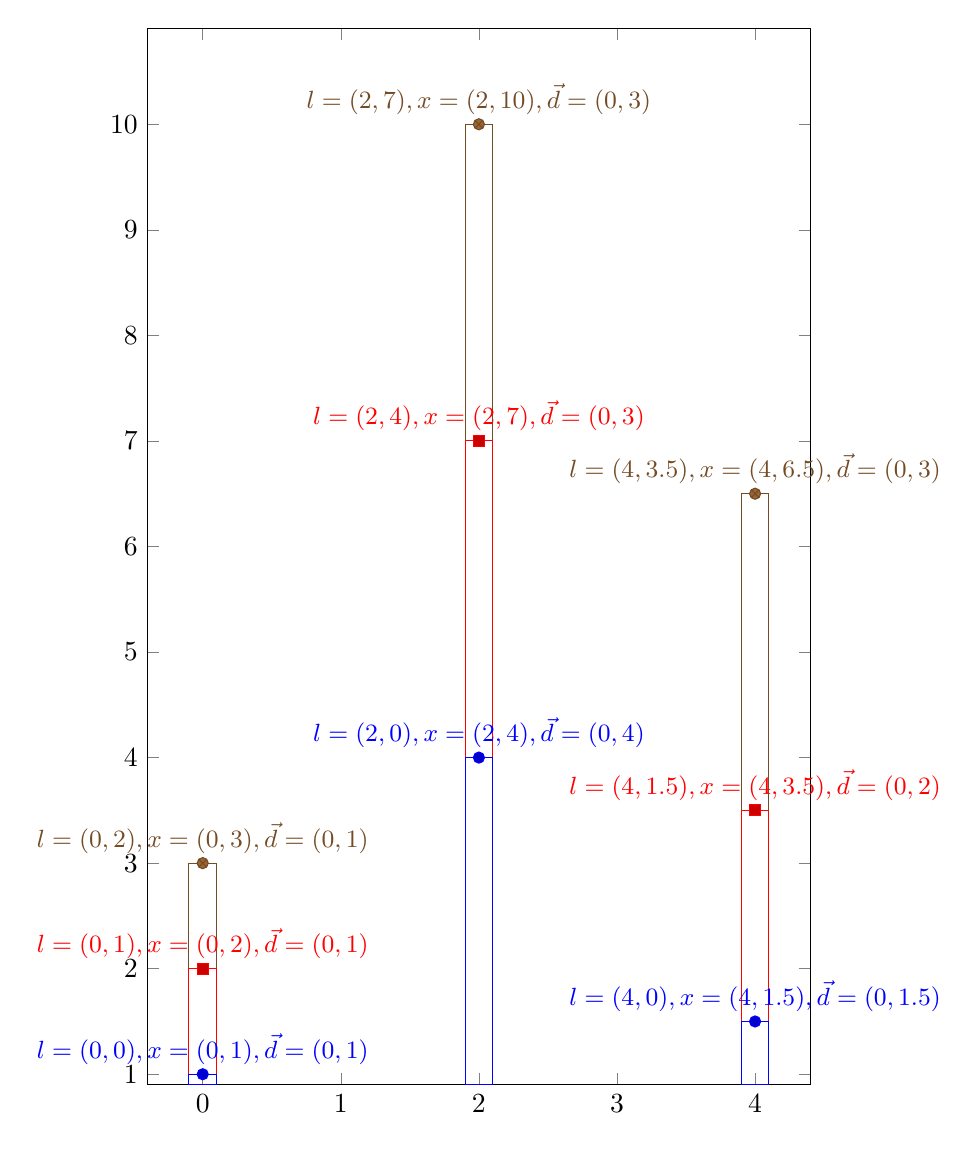
\begin{tikzpicture}
    \begin{axis}[stack plots=y,
		/tikz/ybar,
		height=15cm,
		width=10cm,
		ymin=0.9,
		nodes near coords={%
			\small
			\pgfplotspointgetcoordinates
			\pgfplotspointgetzerolevelcoordinates
			$l = (
				\pgfmathprintnumber{\pgfkeysvalueof{/data point/zero/x}},
				\pgfmathprintnumber{\pgfkeysvalueof{/data point/zero/y}})
			, x = (
				\pgfmathprintnumber{\pgfkeysvalueof{/data point/x}},
				\pgfmathprintnumber{\pgfkeysvalueof{/data point/y}})
			, \vec d = (
				\pgfmathprintnumber{\pgfkeysvalueof{/data point/diff/x}},
				\pgfmathprintnumber{\pgfkeysvalueof{/data point/diff/y}})
		 $},
	]
    \addplot coordinates
        {(0,1) (2,4) (4,1.5)};
    \addplot coordinates
        {(0,1) (2,3) (4,2)};
    \addplot coordinates
        {(0,1) (2,3) (4,3)};
    \end{axis}
\end{tikzpicture}

\end{document}

